\subsection{Esquema alternativo} % (fold)
\label{sub:esq-alt}
El esquema propuesto en esta subsección se debe a la forma en que están 
organizados los datasets que se usan en el entrenamiento y \textit{testing} 
de los algoritmos de reconocimiento de objetos. Se puede consultar DBpedia
(\url{https://wiki.dbpedia.org}) para percatarse de la forma tan 
sistemática y jerarquizada  de organizar las colecciones de datos, las
clasificaciones más externas ordenan la información en seis grandes clases 
\cite{dbpedia}

\begin{itemize}
    \item Recursos
    \item Personas
    \item Lugares
    \item Trabajo
    \item Especies
    \item Organizaciones
\end{itemize}

Por lo anterior, en es esta parte del trabajo se planea la posibilidad de 
agregar algunos atributos adicionales al objeto con la finalidad de adaptarse 
mejor a la organización de un dataset proporcionado por fuentes de datos como 
DBPedia, COCO dataset, etc. Para ello se le agregan los siguientes atributos 
al elemento \textit{objeto}:

\begin{itemize}
    \item Blandura (softness)
    \item Material primario de construcción (building\_mat)
    \item Color más probable (more\_likely\_color)
\end{itemize}

La ventaja de utilizar Grakn es que es posible agregar tantos atributos como se 
necesiten y en el momento en que se necesiten y con pocas líneas de código, 
como se muestra en 
listing \ref{lst:script7}.

\lstinputlisting[language=Python, firstline=22, lastline=44,
caption=Objeto con varios atributos,label={lst:script7}]{code/schema-modif.gql}

% Aunque la herramienta Grakn es capaz de procesar todos los datos que 
% ingresemos en él, es importante señalar que demasiada información podría traer 
% de vuelta el problema que se trata de mitigar (la lentitud). Así mismo esto se 
% ve reflejado a la hora de dibujar el grafo en pantalla, como se observa en la 
% figura \ref{fig:mess}, no es sencillo identificar las relaciones
% si se desea procesar toda la información en una sola consulta.

% \begin{figure}[H]
%     \centering
%     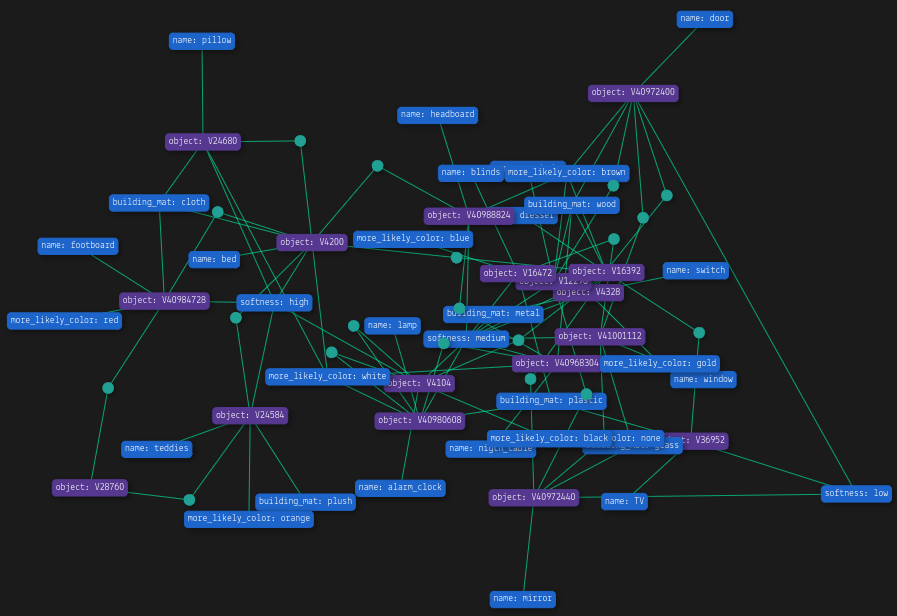
\includegraphics[width=8cm]{figures/problem.png}
%     \caption{Grafo Esperado con demasiadas relaciones para ser leído}
%     \label{fig:mess}
% \end{figure}